% Options for packages loaded elsewhere
\PassOptionsToPackage{unicode}{hyperref}
\PassOptionsToPackage{hyphens}{url}
%
\documentclass[
]{book}
\usepackage{amsmath,amssymb}
\usepackage{lmodern}
\usepackage{iftex}
\ifPDFTeX
  \usepackage[T1]{fontenc}
  \usepackage[utf8]{inputenc}
  \usepackage{textcomp} % provide euro and other symbols
\else % if luatex or xetex
  \usepackage{unicode-math}
  \defaultfontfeatures{Scale=MatchLowercase}
  \defaultfontfeatures[\rmfamily]{Ligatures=TeX,Scale=1}
  \setmainfont[]{NanumGothic}
\fi
% Use upquote if available, for straight quotes in verbatim environments
\IfFileExists{upquote.sty}{\usepackage{upquote}}{}
\IfFileExists{microtype.sty}{% use microtype if available
  \usepackage[]{microtype}
  \UseMicrotypeSet[protrusion]{basicmath} % disable protrusion for tt fonts
}{}
\makeatletter
\@ifundefined{KOMAClassName}{% if non-KOMA class
  \IfFileExists{parskip.sty}{%
    \usepackage{parskip}
  }{% else
    \setlength{\parindent}{0pt}
    \setlength{\parskip}{6pt plus 2pt minus 1pt}}
}{% if KOMA class
  \KOMAoptions{parskip=half}}
\makeatother
\usepackage{xcolor}
\usepackage{color}
\usepackage{fancyvrb}
\newcommand{\VerbBar}{|}
\newcommand{\VERB}{\Verb[commandchars=\\\{\}]}
\DefineVerbatimEnvironment{Highlighting}{Verbatim}{commandchars=\\\{\}}
% Add ',fontsize=\small' for more characters per line
\usepackage{framed}
\definecolor{shadecolor}{RGB}{248,248,248}
\newenvironment{Shaded}{\begin{snugshade}}{\end{snugshade}}
\newcommand{\AlertTok}[1]{\textcolor[rgb]{0.94,0.16,0.16}{#1}}
\newcommand{\AnnotationTok}[1]{\textcolor[rgb]{0.56,0.35,0.01}{\textbf{\textit{#1}}}}
\newcommand{\AttributeTok}[1]{\textcolor[rgb]{0.77,0.63,0.00}{#1}}
\newcommand{\BaseNTok}[1]{\textcolor[rgb]{0.00,0.00,0.81}{#1}}
\newcommand{\BuiltInTok}[1]{#1}
\newcommand{\CharTok}[1]{\textcolor[rgb]{0.31,0.60,0.02}{#1}}
\newcommand{\CommentTok}[1]{\textcolor[rgb]{0.56,0.35,0.01}{\textit{#1}}}
\newcommand{\CommentVarTok}[1]{\textcolor[rgb]{0.56,0.35,0.01}{\textbf{\textit{#1}}}}
\newcommand{\ConstantTok}[1]{\textcolor[rgb]{0.00,0.00,0.00}{#1}}
\newcommand{\ControlFlowTok}[1]{\textcolor[rgb]{0.13,0.29,0.53}{\textbf{#1}}}
\newcommand{\DataTypeTok}[1]{\textcolor[rgb]{0.13,0.29,0.53}{#1}}
\newcommand{\DecValTok}[1]{\textcolor[rgb]{0.00,0.00,0.81}{#1}}
\newcommand{\DocumentationTok}[1]{\textcolor[rgb]{0.56,0.35,0.01}{\textbf{\textit{#1}}}}
\newcommand{\ErrorTok}[1]{\textcolor[rgb]{0.64,0.00,0.00}{\textbf{#1}}}
\newcommand{\ExtensionTok}[1]{#1}
\newcommand{\FloatTok}[1]{\textcolor[rgb]{0.00,0.00,0.81}{#1}}
\newcommand{\FunctionTok}[1]{\textcolor[rgb]{0.00,0.00,0.00}{#1}}
\newcommand{\ImportTok}[1]{#1}
\newcommand{\InformationTok}[1]{\textcolor[rgb]{0.56,0.35,0.01}{\textbf{\textit{#1}}}}
\newcommand{\KeywordTok}[1]{\textcolor[rgb]{0.13,0.29,0.53}{\textbf{#1}}}
\newcommand{\NormalTok}[1]{#1}
\newcommand{\OperatorTok}[1]{\textcolor[rgb]{0.81,0.36,0.00}{\textbf{#1}}}
\newcommand{\OtherTok}[1]{\textcolor[rgb]{0.56,0.35,0.01}{#1}}
\newcommand{\PreprocessorTok}[1]{\textcolor[rgb]{0.56,0.35,0.01}{\textit{#1}}}
\newcommand{\RegionMarkerTok}[1]{#1}
\newcommand{\SpecialCharTok}[1]{\textcolor[rgb]{0.00,0.00,0.00}{#1}}
\newcommand{\SpecialStringTok}[1]{\textcolor[rgb]{0.31,0.60,0.02}{#1}}
\newcommand{\StringTok}[1]{\textcolor[rgb]{0.31,0.60,0.02}{#1}}
\newcommand{\VariableTok}[1]{\textcolor[rgb]{0.00,0.00,0.00}{#1}}
\newcommand{\VerbatimStringTok}[1]{\textcolor[rgb]{0.31,0.60,0.02}{#1}}
\newcommand{\WarningTok}[1]{\textcolor[rgb]{0.56,0.35,0.01}{\textbf{\textit{#1}}}}
\usepackage{longtable,booktabs,array}
\usepackage{calc} % for calculating minipage widths
% Correct order of tables after \paragraph or \subparagraph
\usepackage{etoolbox}
\makeatletter
\patchcmd\longtable{\par}{\if@noskipsec\mbox{}\fi\par}{}{}
\makeatother
% Allow footnotes in longtable head/foot
\IfFileExists{footnotehyper.sty}{\usepackage{footnotehyper}}{\usepackage{footnote}}
\makesavenoteenv{longtable}
\usepackage{graphicx}
\makeatletter
\def\maxwidth{\ifdim\Gin@nat@width>\linewidth\linewidth\else\Gin@nat@width\fi}
\def\maxheight{\ifdim\Gin@nat@height>\textheight\textheight\else\Gin@nat@height\fi}
\makeatother
% Scale images if necessary, so that they will not overflow the page
% margins by default, and it is still possible to overwrite the defaults
% using explicit options in \includegraphics[width, height, ...]{}
\setkeys{Gin}{width=\maxwidth,height=\maxheight,keepaspectratio}
% Set default figure placement to htbp
\makeatletter
\def\fps@figure{htbp}
\makeatother
\setlength{\emergencystretch}{3em} % prevent overfull lines
\providecommand{\tightlist}{%
  \setlength{\itemsep}{0pt}\setlength{\parskip}{0pt}}
\setcounter{secnumdepth}{5}
\usepackage{booktabs}
\ifLuaTeX
  \usepackage{selnolig}  % disable illegal ligatures
\fi
\usepackage[]{natbib}
\bibliographystyle{apalike}
\IfFileExists{bookmark.sty}{\usepackage{bookmark}}{\usepackage{hyperref}}
\IfFileExists{xurl.sty}{\usepackage{xurl}}{} % add URL line breaks if available
\urlstyle{same} % disable monospaced font for URLs
\hypersetup{
  pdftitle={2022년 한국생명공학연구원 연구데이터 분석과정 R},
  pdfauthor={합성생물학전문연구단 김하성},
  hidelinks,
  pdfcreator={LaTeX via pandoc}}

\title{2022년 한국생명공학연구원 연구데이터 분석과정 R}
\author{합성생물학전문연구단 김하성}
\date{2022-05-18}

\begin{document}
\maketitle

{
\setcounter{tocdepth}{1}
\tableofcontents
}
\hypertarget{introduction}{%
\chapter{Introduction}\label{introduction}}

\hypertarget{Information}{%
\section{강의 개요}\label{Information}}

\begin{itemize}
\tightlist
\item
  목표: 생물 데이터 분석을 위한 R 사용법과 (Rstudio, Tidyverse, Bioconductor 포함) 프로그래밍 기술을 습득함
\item
  장소: 코빅 3층 전산교육장(1304호)
\item
  강사: 한국생명공학연구원 합성생물학전문연구단 김하성
\item
  연락처: 042-860-4372, \href{mailto:haseong@kribb.re.kr}{\nolinkurl{haseong@kribb.re.kr}}
\item
  강의자료: \url{https://greendaygh.github.io/kribb2022R/}
\end{itemize}

\hypertarget{Schedule}{%
\section{강의 계획}\label{Schedule}}

\begin{enumerate}
\def\labelenumi{\arabic{enumi}.}
\tightlist
\item
  R 사용법 및 데이터 분석 기초 5.19(목), 5.26(목)
\item
  R/Tidyverse 데이터 분석 중급 6.9(목), 6.16(목)
\item
  R/Tidyverse 활용 데이터 가시화 7.7(목), 7.14(목)
\item
  R/Bioconductor 활용한 바이오데이터 분석 기초 8.4(목), 8.11(목)
\item
  R/Bioconductor 활용한 NGS 데이터 분석 기초 9.1(목), 9.15(목)
\item
  R/Bioconductor 활용한 NGS 데이터 분석 및 Workflow 10.6(목), 10.13(목)
\end{enumerate}

\hypertarget{References}{%
\section{참고 자료}\label{References}}

\begin{itemize}
\tightlist
\item
  \href{https://www.r-project.org/}{R 홈페이지}
\item
  \href{https://www.rstudio.com/}{Rstudio 홈페이지}
\item
  \href{https://www.bioconductor.org/}{Bioconductor}
\item
  \href{https://cran.r-project.org/manuals.html}{R 기본 문서들}
\item
  \href{https://bookdown.org/}{R ebooks}
\item
  \href{https://www.rstudio.com/resources/cheatsheets/}{Cheat Sheets}
\item
  \href{https://resources.rstudio.com/}{RStudio Webinars}
\item
  \href{http://shiny.rstudio.com/tutorial/}{Shiny}
\item
  \href{https://github.com/hadley}{Hadley github}
\item
  \href{https://r4ds.had.co.nz}{R for Data Science}
\item
  Using R for Introductory Statistics by John Verzani

  \begin{itemize}
  \tightlist
  \item
    Free version of \href{https://cran.r-project.org/doc/contrib/Verzani-SimpleR.pdf}{1st Edition}
  \item
    \href{https://www.crcpress.com/Using-R-for-Introductory-Statistics-Second-Edition/Verzani/p/book/9781466590731}{Second edition}
  \end{itemize}
\item
  \href{http://2.droppdf.com/files/5aTvl/bioinformatics-data-skills.pdf}{Bioinformatics Data Skills} by Vince Buffalo
\item
  \href{http://www.academia.dk/BiologiskAntropologi/Epidemiologi/PDF/Introductory_Statistics_with_R__2nd_ed.pdf}{Introductory Statistics with R} by Dalgaard
\item
  일반통계학 (영지문화사, 김우철 외)
\end{itemize}

\hypertarget{rrstudio-basics}{%
\chapter{R/Rstudio basics}\label{rrstudio-basics}}

\hypertarget{what-is-r-rstudio}{%
\section{What is R / Rstudio}\label{what-is-r-rstudio}}


\includegraphics{images/01/r.jpg}

R은 통계나 생물통계, 유전학을 연구하는 사람들 사이에서 널리 사용되는 오픈소스 프로그래밍 언어 입니다. Bell Lab에서 개발한 S 언어에서 유래했으며 많은 라이브러리 (다른 사람들이 만들어 놓은 코드)가 있어서 쉽게 가져다 사용할 수 있습니다. R은 복잡한 수식이나 통계 알고리즘을 간단히 구현하고 사용할 수 있으며 C, C++, Python 등 다른 언어들과의 병행 사용도 가능합니다. R은 IEEE에서 조사하는 Top programming languages에서 2018년 7위, 2019년 5위, 2020년 6위, 2021년 7위로 꾸준히 높은 사용자를 확보하며 빅데이터, AI 시대의 주요한 프로그래밍 언어로 사용되고 있습니다.

\begin{figure}
\centering
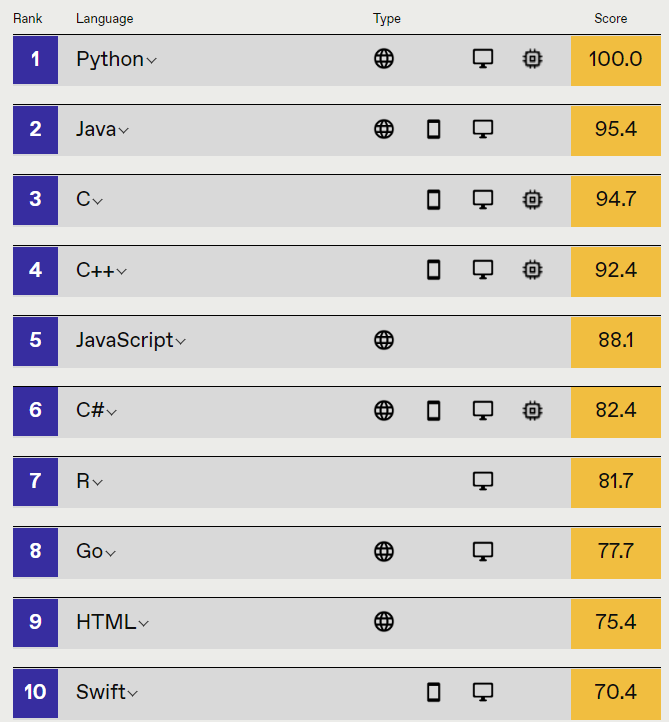
\includegraphics[width=4.6875in,height=\textheight]{images/01/toplanguage2021.png}
\caption{\url{https://spectrum.ieee.org/top-programming-languages/}}
\end{figure}

R은 데이터를 통계분석에 널리 사용되는데 이는 데이터를 눈으로 확인하기 위한 visualization 이나 벡터 연산 등의 강력한 기능 때문에 점점 더 많은 사람들이 사용하고 있습니다. 기존에는 속도나 확장성이 다른 언어들에 비해 단점으로 지적되었으나 R 언어의 계속적인 개발과 업데이트로 이러한 단점들이 빠르게 보완되고 있습니다. R 사용을 위해서는 R 언어의 코어 프로그램을 먼저 설치하고 그 다음 R 언어용 IDE(Integrated Development Environment)인 RStudio 설치가 필요합니다.


\includegraphics{images/01/rstudio.png}

Rstudio는 R 언어를 위한 오픈소스 기반 통합개발환경(IDE)으로 R 프로그래밍을 위한 편리한 기능들을 제공해 줍니다. R언어가 주목을 받고 두터운 사용자 층을 확보할 수 있게된 핵심 동력이 Rstudio 입니다. 자체적으로 최고수준의 오픈소스 개발팀이 있으며 \texttt{tidyverse}, `\texttt{,}shiny` 등의 데이터 분석 관련 주요 패키지를 개발하였고 정기적으로 conference 개최를 하면서 기술 보급의 핵심 역할을 하고 있습니다.

\begin{figure}
\centering
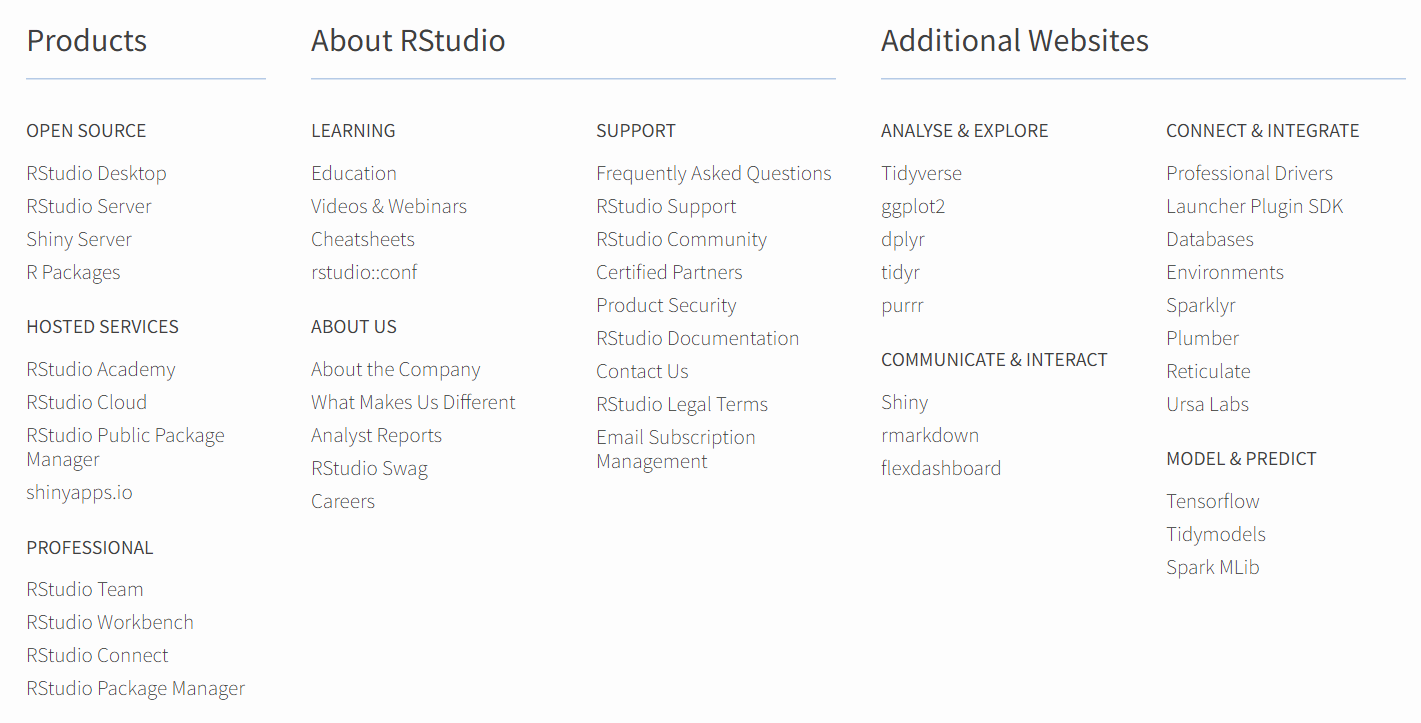
\includegraphics[width=5.72917in,height=\textheight]{images/01/rstudiobottom.png}
\caption{\url{https://www.rstudio.com/}}
\end{figure}

\hypertarget{r-rstudio-installation}{%
\section{R / Rstudio Installation}\label{r-rstudio-installation}}

\hypertarget{r-uxc124uxce58}{%
\subsection{R 설치}\label{r-uxc124uxce58}}

\begin{itemize}
\tightlist
\item
  R 사이트에 접속 후 (\url{https://www.r-project.org/}) 좌측 메뉴 상단에 위치한 CRAN 클릭.
\item
  미러 사이트 목록에서 Korea의 아무 사이트나 들어감
\item
  Download R for Windows를 클릭 후 base 링크 들어가서
\item
  Download R x.x.x for Windows 링크 클릭으로 실행 프로그램 다운로드
\item
  로컬 컴퓨터에 Download 된 R-x.x.x-win.exe 를 실행 (2022.5 현재 R 버전은 4.2.0).
\item
  설치 프로그램의 지시에 따라 R 언어 소프트웨어 설치를 완료
\end{itemize}

\hypertarget{rstudio-uxc124uxce58}{%
\subsection{Rstudio 설치}\label{rstudio-uxc124uxce58}}

\begin{itemize}
\tightlist
\item
  사이트에 접속 (\url{https://www.rstudio.com/}), 상단의 Products \textgreater{} RStudio 클릭
\item
  RStudio Desktop 선택
\item
  Download RStudio Desktop 클릭
\item
  RStudio Desktop Free 버전의 Download를 선택하고
\item
  Download RStudio for Windows 클릭, 다운로드
\item
  로컬 컴퓨터에 다운로드된 RStudio-x.x.x.exe 실행 (2022.5 현재 RStudio Desktop 2022.02.2+485)
\item
  설치 가이드에 따라 설치 완료
\end{itemize}

\hypertarget{rstudio-interface}{%
\section{Rstudio interface}\label{rstudio-interface}}

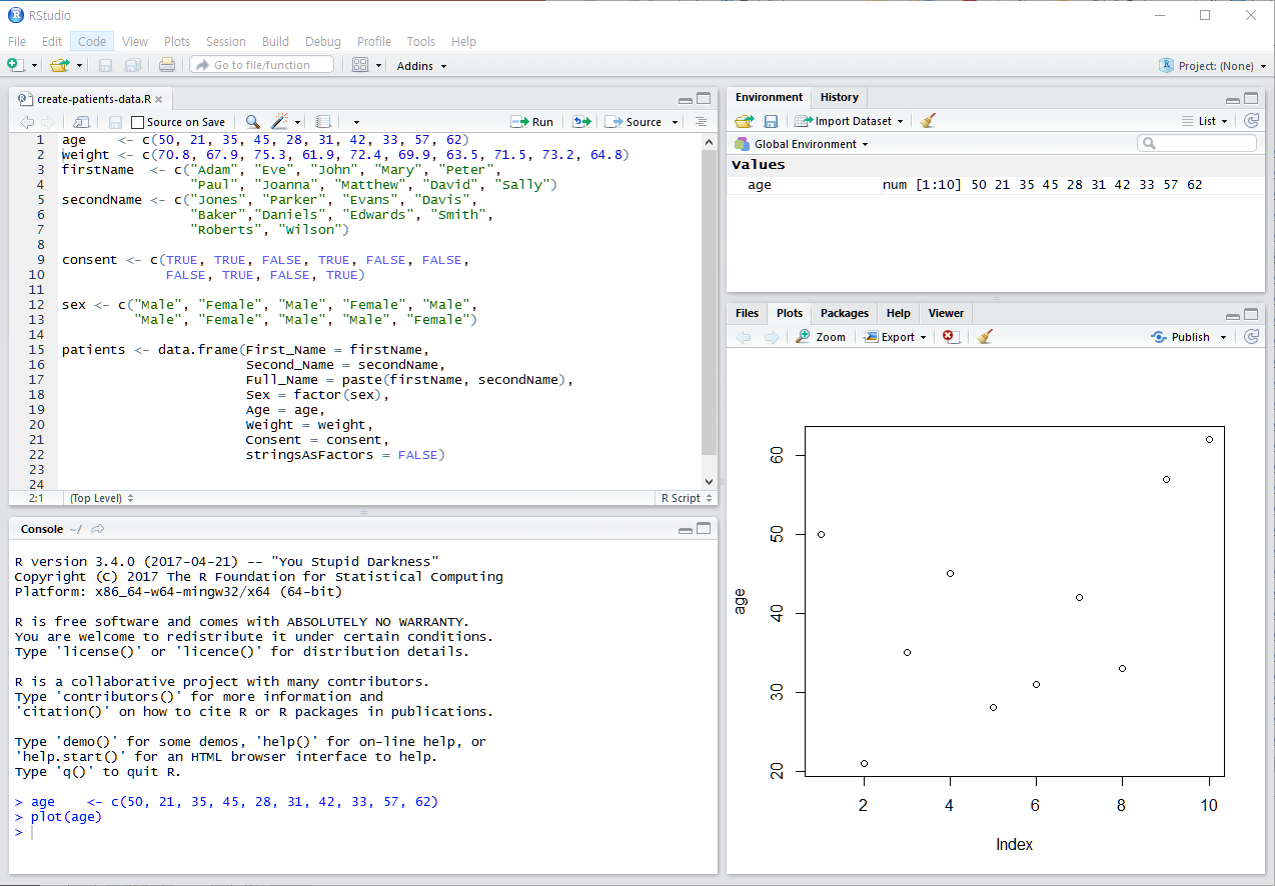
\includegraphics[width=6.77083in,height=\textheight]{images/01/01-11.PNG}

\begin{itemize}
\tightlist
\item
  기본 화면에서 좌측 상단의 공간은 코드편집창, 좌측 하단은 콘솔창
\item
  각 위치를 기호에 따라서 바꿀 수 있음 (View --\textgreater{} Pane)
\end{itemize}

\hypertarget{keyboard-shortcuts}{%
\subsection{Keyboard shortcuts}\label{keyboard-shortcuts}}

\begin{itemize}
\tightlist
\item
  참고사이트

  \begin{itemize}
  \tightlist
  \item
    \url{https://support.rstudio.com/hc/en-us/articles/200711853-Keyboard-Shortcuts}
  \item
    Tools --\textgreater{} Keyboard shortcut Quick Reference (\texttt{Alt\ +\ Shift\ +\ K})
  \end{itemize}
\item
  코드편집창 이동 (\texttt{Ctrl\ +\ 1}) 콘솔창 이동(\texttt{Ctrl\ +\ 2})
\item
  한 줄 실행 (\texttt{Ctrl\ +\ Enter})
\item
  저장 (\texttt{Ctrl\ +\ S})
\item
  주석처리 (\texttt{Ctrl\ +\ Shift\ +\ C})

  \begin{itemize}
  \tightlist
  \item
    또는 \texttt{\#}으로 시작하는 라인
  \end{itemize}
\item
  텝 이동 (\texttt{Ctrl\ +\ F11}, \texttt{Ctrl\ +\ F12})
\item
  코드편집창 확대 (\texttt{Shift\ +\ Ctrl\ +\ 1}) 콘솔창 확대 (\texttt{Shift\ +\ Ctrl\ +\ 2})
\item
  컬럼 편집 (\texttt{Alt\ +\ 마우스\ 드레그})
\end{itemize}

\hypertarget{exercise}{%
\subsection{Exercise}\label{exercise}}

\begin{enumerate}
\def\labelenumi{\arabic{enumi}.}
\tightlist
\item
  코드편집창에서 다음을 입력/실행하고 단축키를 사용하여 주석을 넣으시오
\end{enumerate}

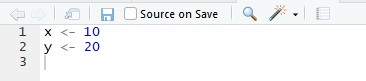
\includegraphics{images/01/01-14.PNG}

\begin{itemize}
\tightlist
\item
  단축키 \texttt{Ctrl\ +\ enter}로 코드 실행
\item
  단축키 \texttt{Ctrl\ +\ 2}로 커서 콘솔창으로 이동
\item
  \texttt{x}값 \texttt{x+y}값 확인
\item
  단축키 \texttt{Ctrl\ +\ 1}로 코드편집창 이동
\item
  단축키 \texttt{Ctrl\ +\ Shift\ +\ C} 사용
\end{itemize}

\begin{Shaded}
\begin{Highlighting}[]
\CommentTok{\# x \textless{}{-} 10}
\CommentTok{\# y \textless{}{-} 20}
\end{Highlighting}
\end{Shaded}

\hypertarget{set-a-project}{%
\subsection{Set a project}\label{set-a-project}}

프로젝트를 만들어서 사용할 경우 파일이나 디렉토리, 내용 등을 쉽게 구분하여 사용 가능합니다. 아래와 같이 임의의 디렉토리에 \texttt{kribbR} 이라는 디렉토리를 생성하고 \texttt{lecture1} 프로젝트를 만듭니다.

\begin{quote}
File \textgreater{} New Project \textgreater{} New Directory \textgreater{} New Project \textgreater{} ``kribbR'' \textgreater{} Create Project
\end{quote}

시작할 때는 해당 디렉토리의 \texttt{xxx.Rproj} 파일을 클릭합니다. Rstudio 오른쪽 상단 프로젝트 선택을 통해서 빠르게 다른 프로젝트의 작업공간으로 이동할 수 있습니다.

\hypertarget{terminology}{%
\subsection{Terminology}\label{terminology}}

\begin{itemize}
\tightlist
\item
  Session: R 언어 실행 환경
\item
  Console: 명령어 입력하는 창
\item
  Code: R 프로그래밍 변수/제어문 모음
\item
  Object types:

  \begin{itemize}
  \tightlist
  \item
    vector: 값들의 모임 combine function \texttt{c()} EX: c(6, 11, 13, 31, 90, 92)
  \item
    matrix: 2D 형태 값들의 모임
  \item
    array: 1D, 2D, 3D, \ldots{} 형태 값들의 모임
  \item
    factor: 범주형 데이터
  \item
    data frame: 2D 형태 값들의 모임 (다른 타입 값 가능)
  \item
    list:
  \item
    function: 특정 기능 수행, {[}함수이름, 입력값 (arguments), 출력값 (return){]} 으로 구성
  \end{itemize}
\item
  Data (value) types:

  \begin{itemize}
  \tightlist
  \item
    Integers
  \item
    doubles/numerics
  \item
    logicals
  \item
    characters.
  \end{itemize}
\item
  Conditionals (조건, 제어):

  \begin{itemize}
  \tightlist
  \item
    \texttt{if}, \texttt{==}, \texttt{\&} (AND), \texttt{\textbar{}} (OR) Ex: \texttt{(2\ +\ 1\ ==\ 3)\ \&\ (2\ +\ 1\ ==\ 4)}
  \item
    \texttt{for}, \texttt{while}: 반복 수
  \end{itemize}
\end{itemize}

\hypertarget{getting-help}{%
\section{Getting help}\label{getting-help}}

R은 방대한 양의 도움말 데이터를 제공하며 다음과 같은 명령어로 특정 함수의 도움말과 예제를 찾아볼 수 있습니다.

\begin{Shaded}
\begin{Highlighting}[]
\FunctionTok{help}\NormalTok{(}\StringTok{"mean"}\NormalTok{)}
\NormalTok{?mean}
\FunctionTok{example}\NormalTok{(}\StringTok{"mean"}\NormalTok{)}
\FunctionTok{help.search}\NormalTok{(}\StringTok{"mean"}\NormalTok{)}
\NormalTok{??mean}
\FunctionTok{help}\NormalTok{(}\AttributeTok{package=}\StringTok{"MASS"}\NormalTok{)}
\end{Highlighting}
\end{Shaded}

또한 \url{https://www.rstudio.com/resources/cheatsheets/} 에서는 다양한 R언어의 기능을 한 눈에 알아볼 수 있게 만든 cheatsheet 형태의 문서를 참고할 수 있습니다.

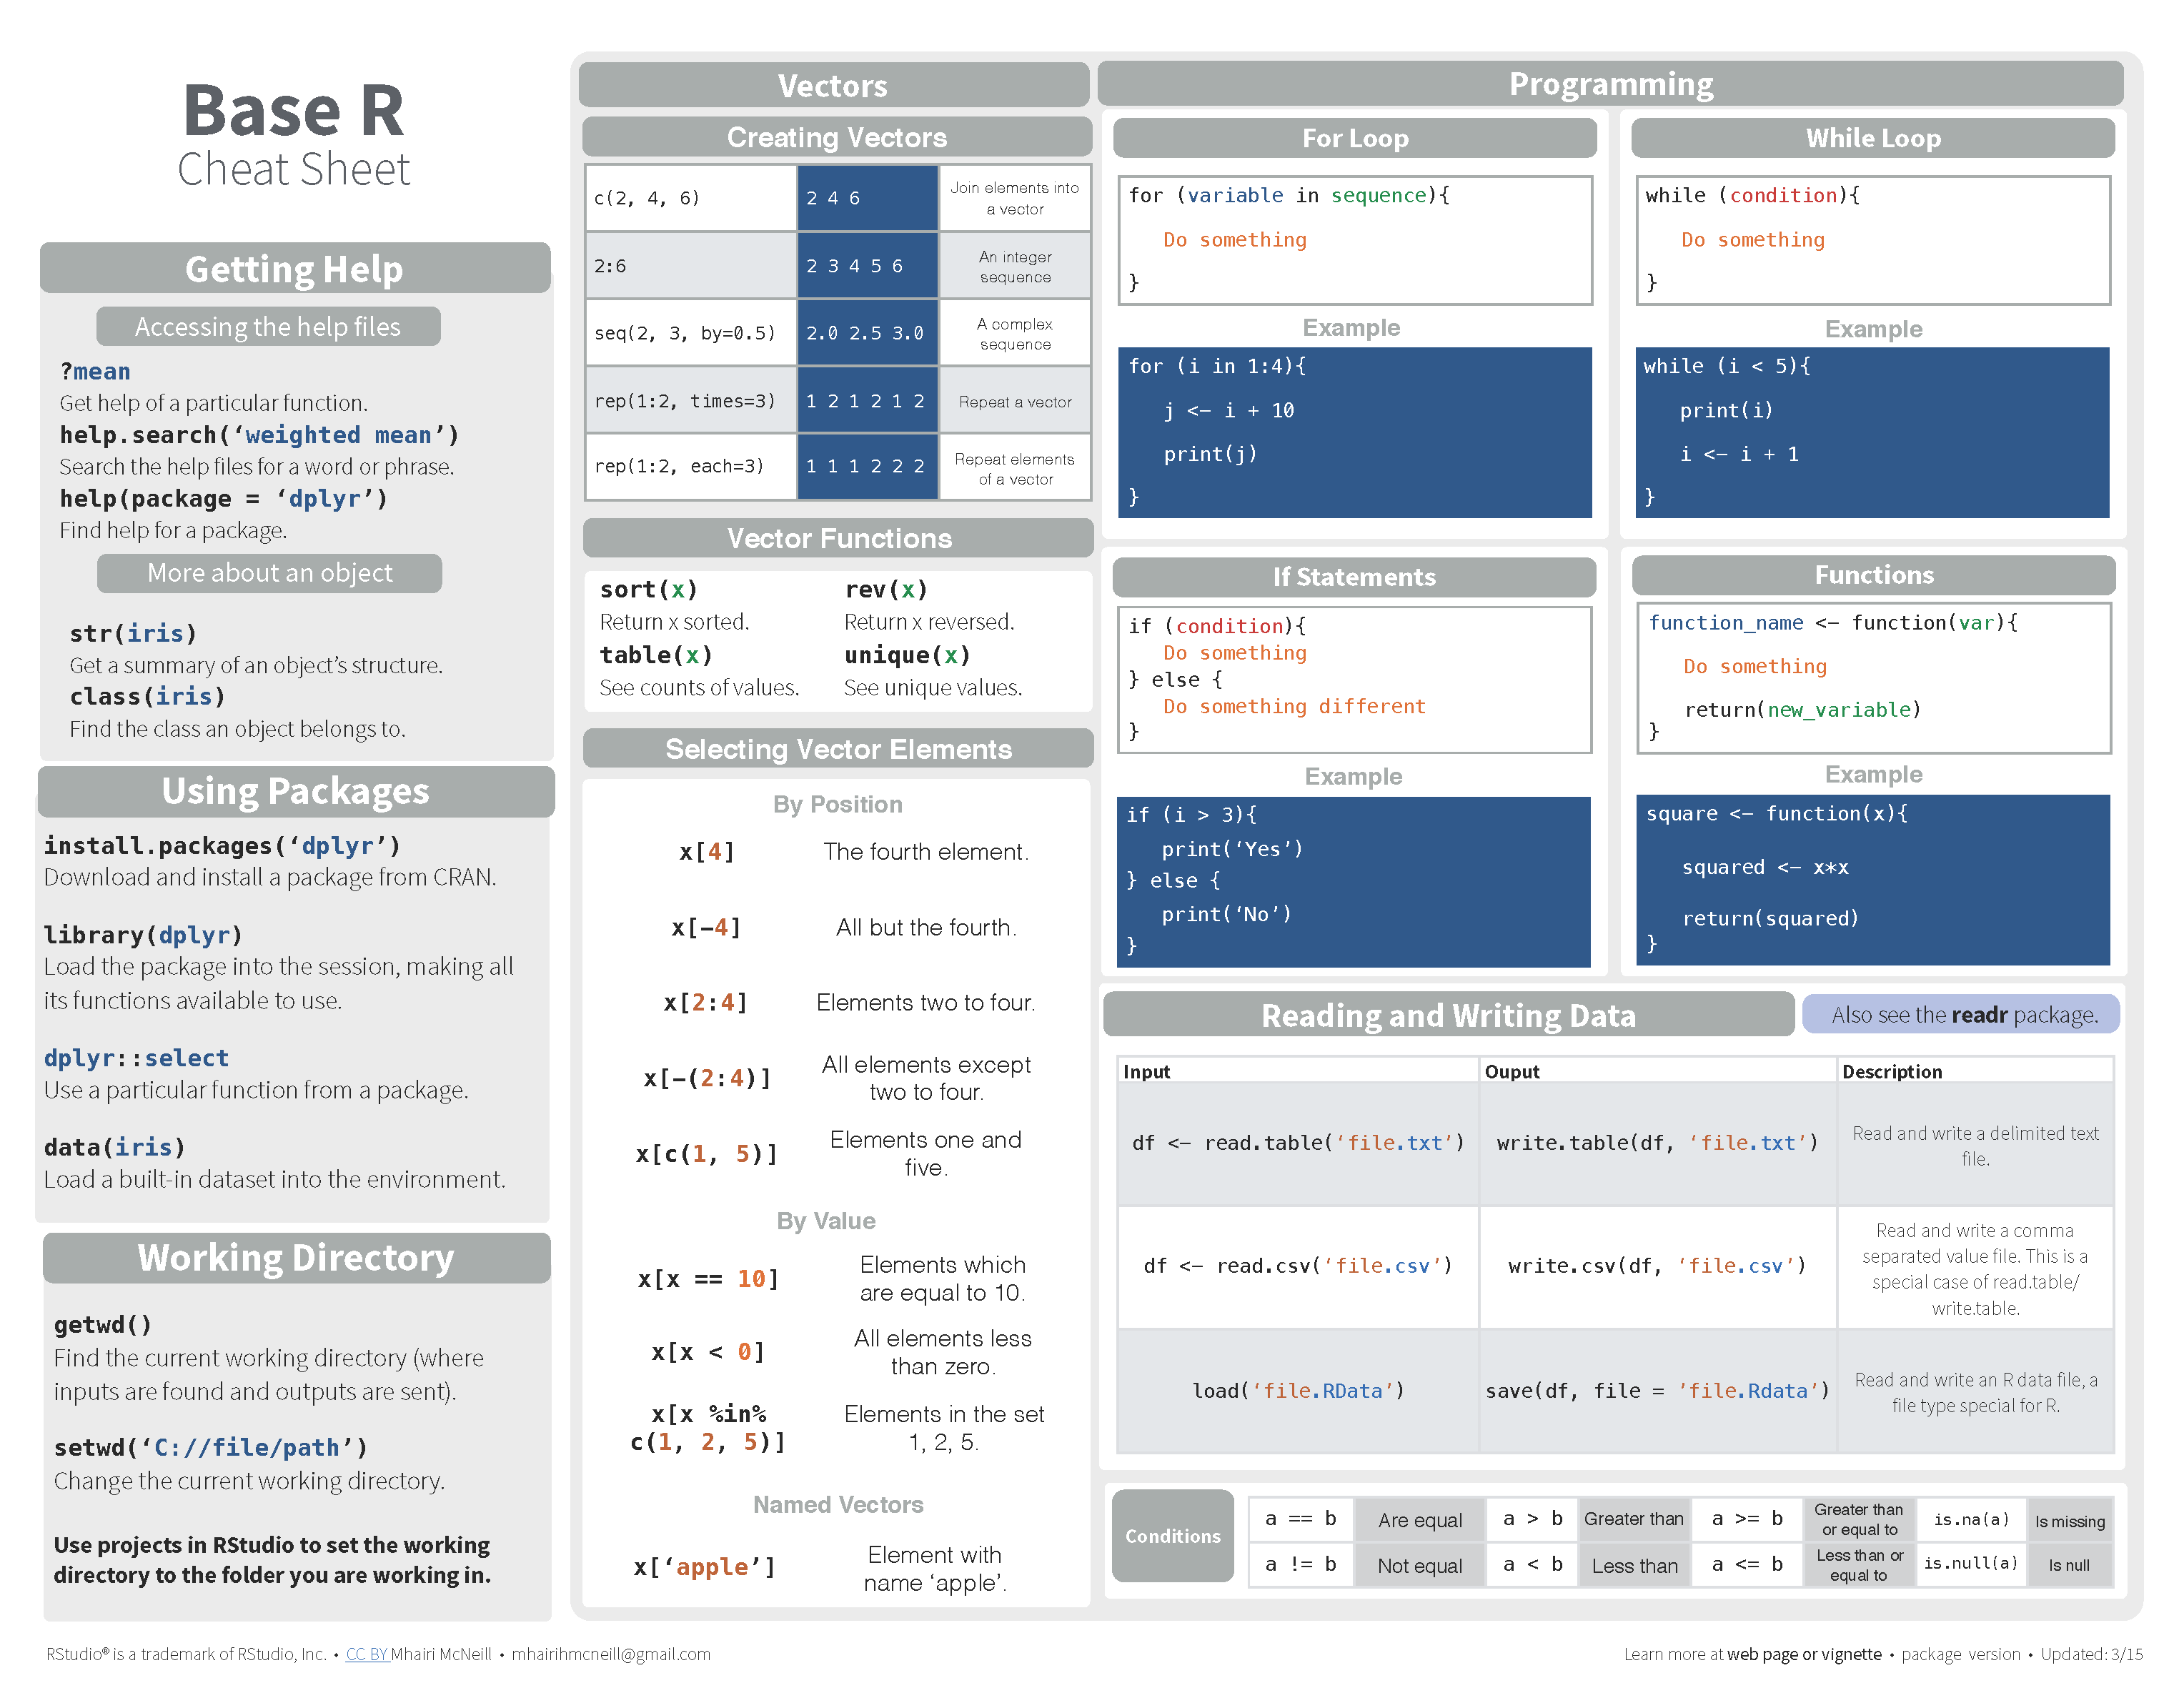
\includegraphics[width=6.77083in,height=\textheight]{images/01/base-r_1.png}
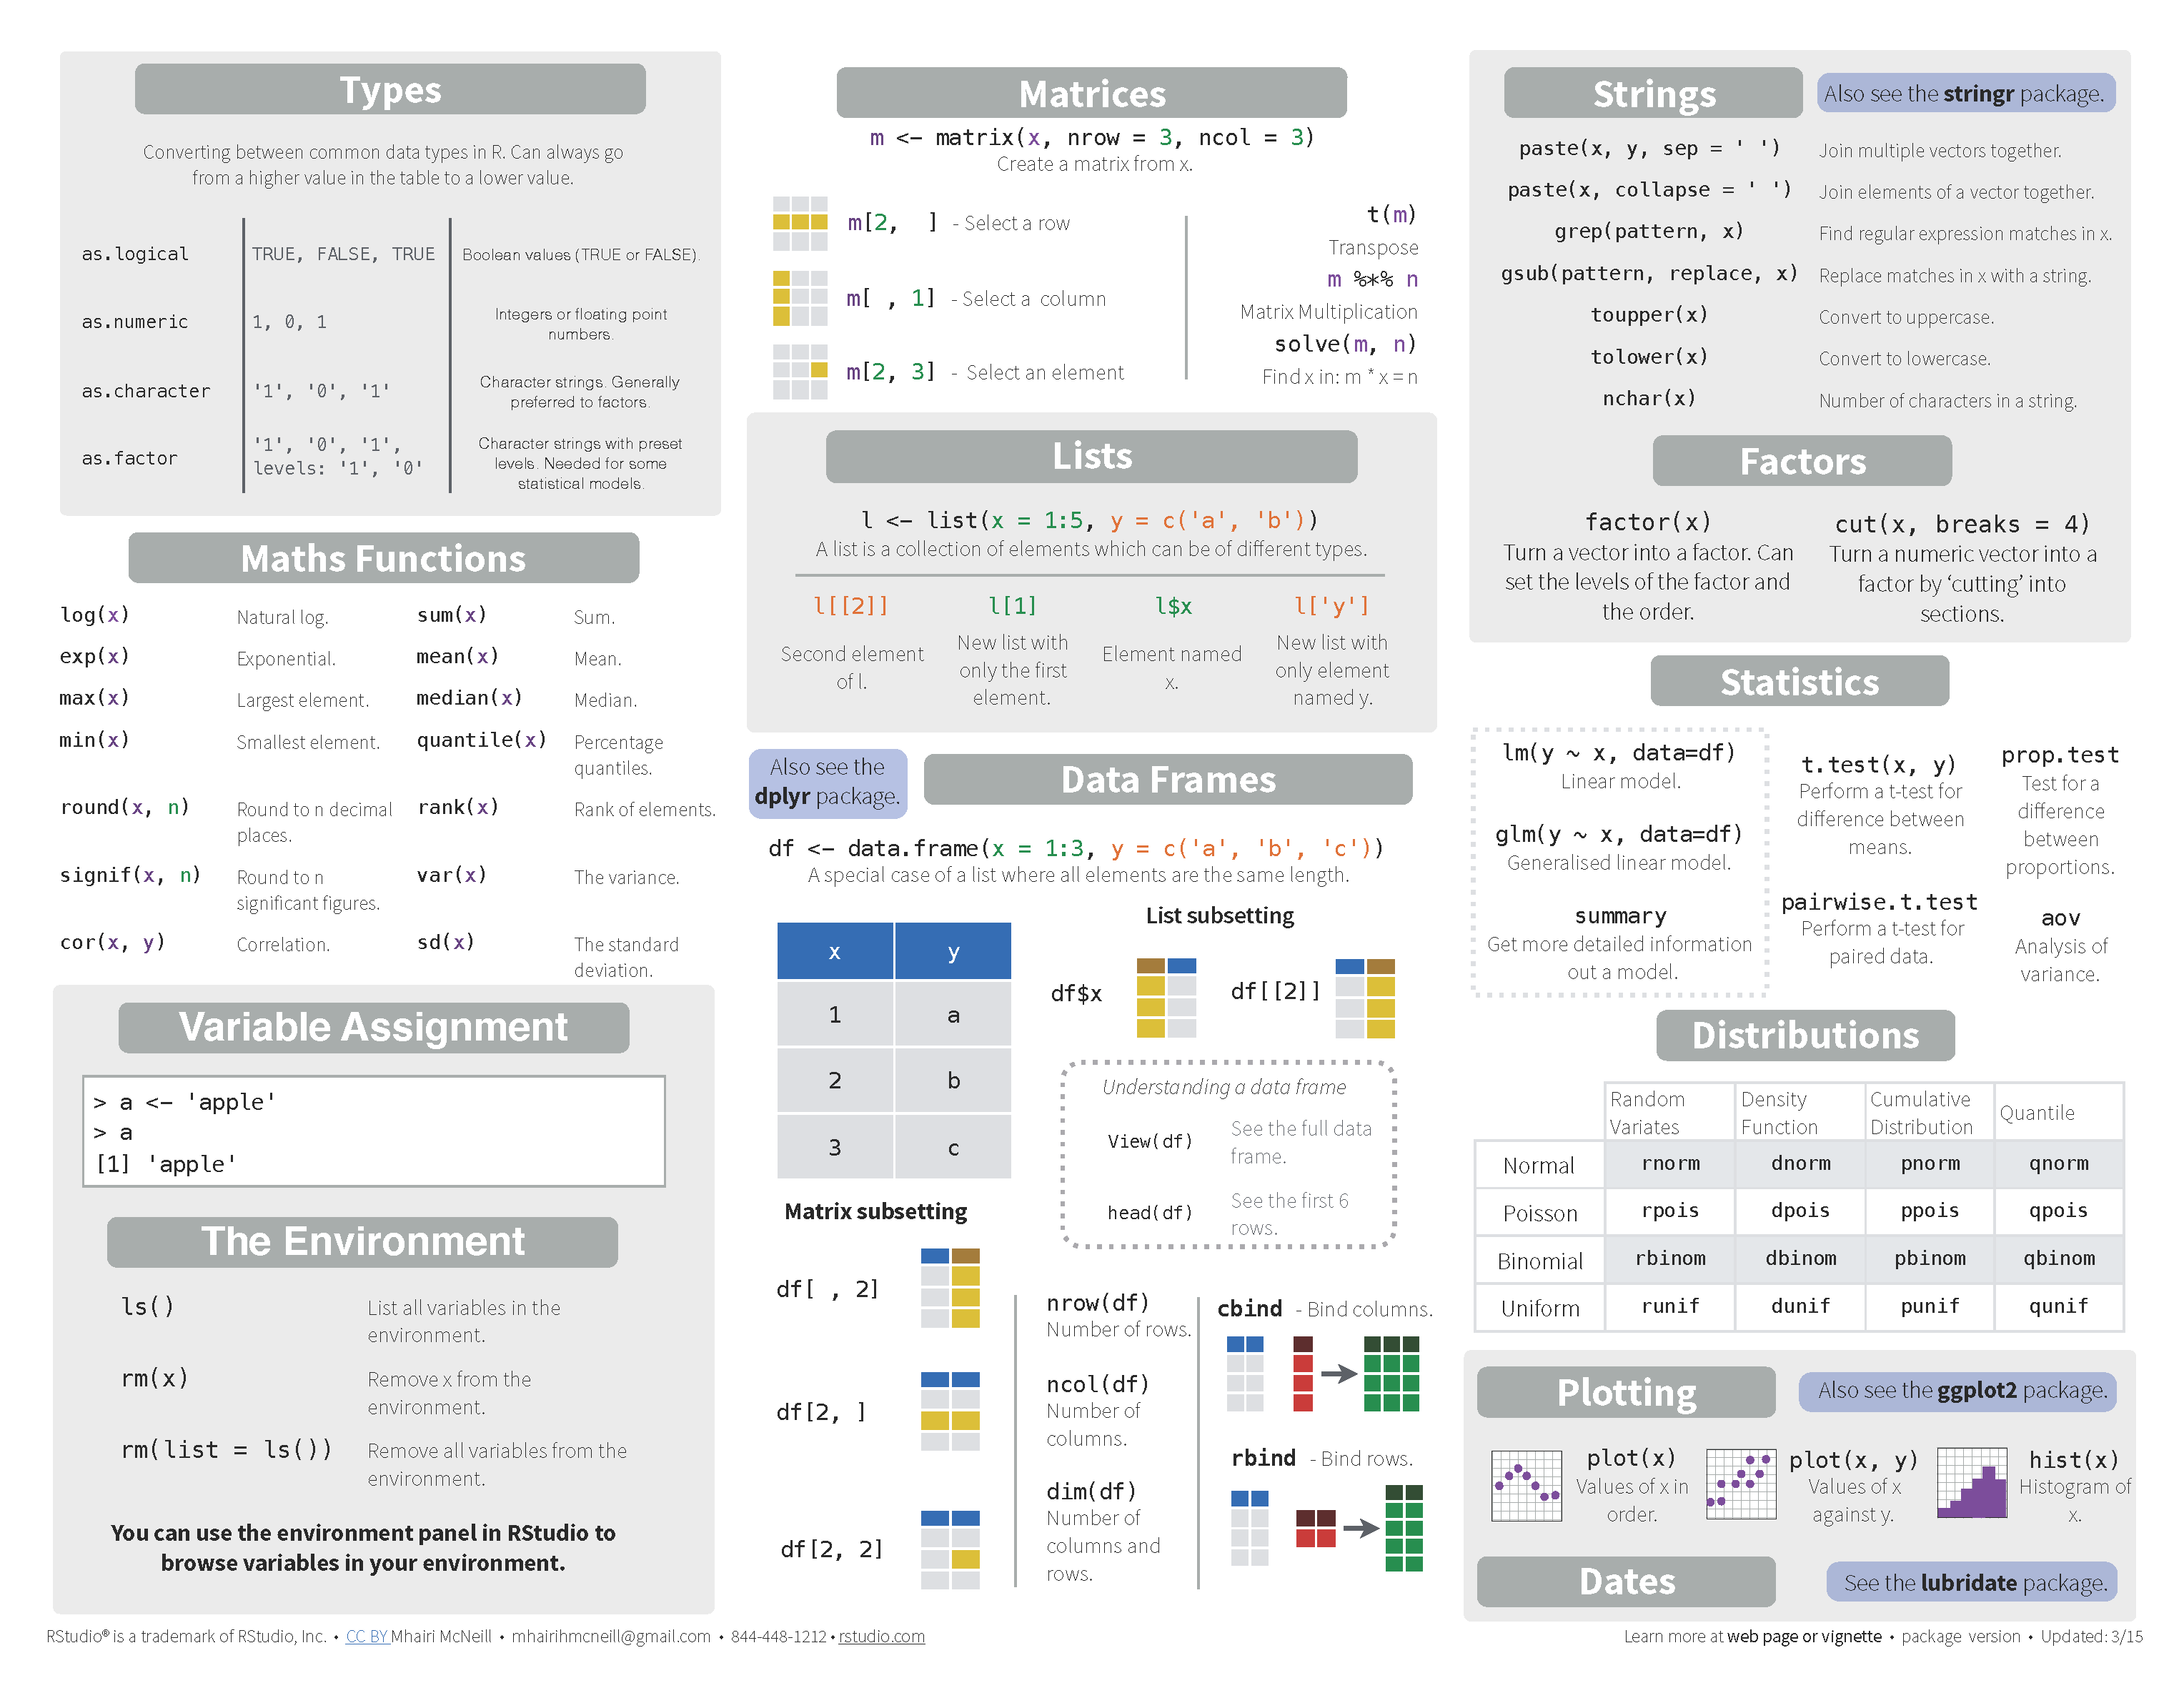
\includegraphics[width=6.77083in,height=\textheight]{images/01/base-r_2.png}

\hypertarget{r-packages-and-dataset}{%
\section{R packages and Dataset}\label{r-packages-and-dataset}}

R 패키지는 함수와 데이터셋의 묶음으로 다른 사람들이 만들어 놓은 코드나 기능을 가져와서 사용하므로써 코드 작성의 수고로움을 줄이고 편리하고 검증된 함수(기능)를 빠르게 도입하여 사용할 수 있다는 장점이 있습니다. 예를 들어 \texttt{sd()} 함수는 \texttt{stats} package에서 제공하는 함수로써 표준편차 계산을 위한 별도의 함수를 만들어서 사용할 필요가 없이 바로 (stats 패키지는 R 기본 패키지로) 별도 설치 없이 바로 사용 가능합니다.

패키지를 구할 수 있는 가장 대표적인 사이트는 (저장소는) The Comprehensive R Archive Network (CRAN) \url{http://cran.r-project.org/web/views/} 이며 우리가 사용할 Bioconductor - \url{http://www.bioconductor.org/packages/release/bioc/} 저장소도 체계적으로 관리되고 많은 사람들이 활용하고 있는 사이트 중 하나입니다.

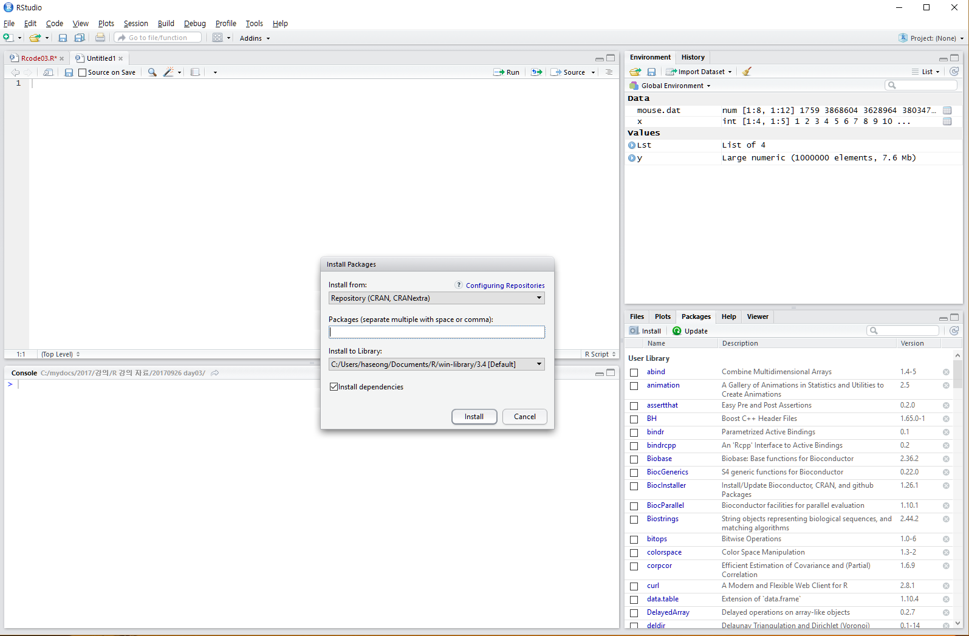
\includegraphics[width=3.64583in,height=\textheight]{images/01/01-18.png}

\begin{itemize}
\tightlist
\item
  UsingR package installation
\end{itemize}

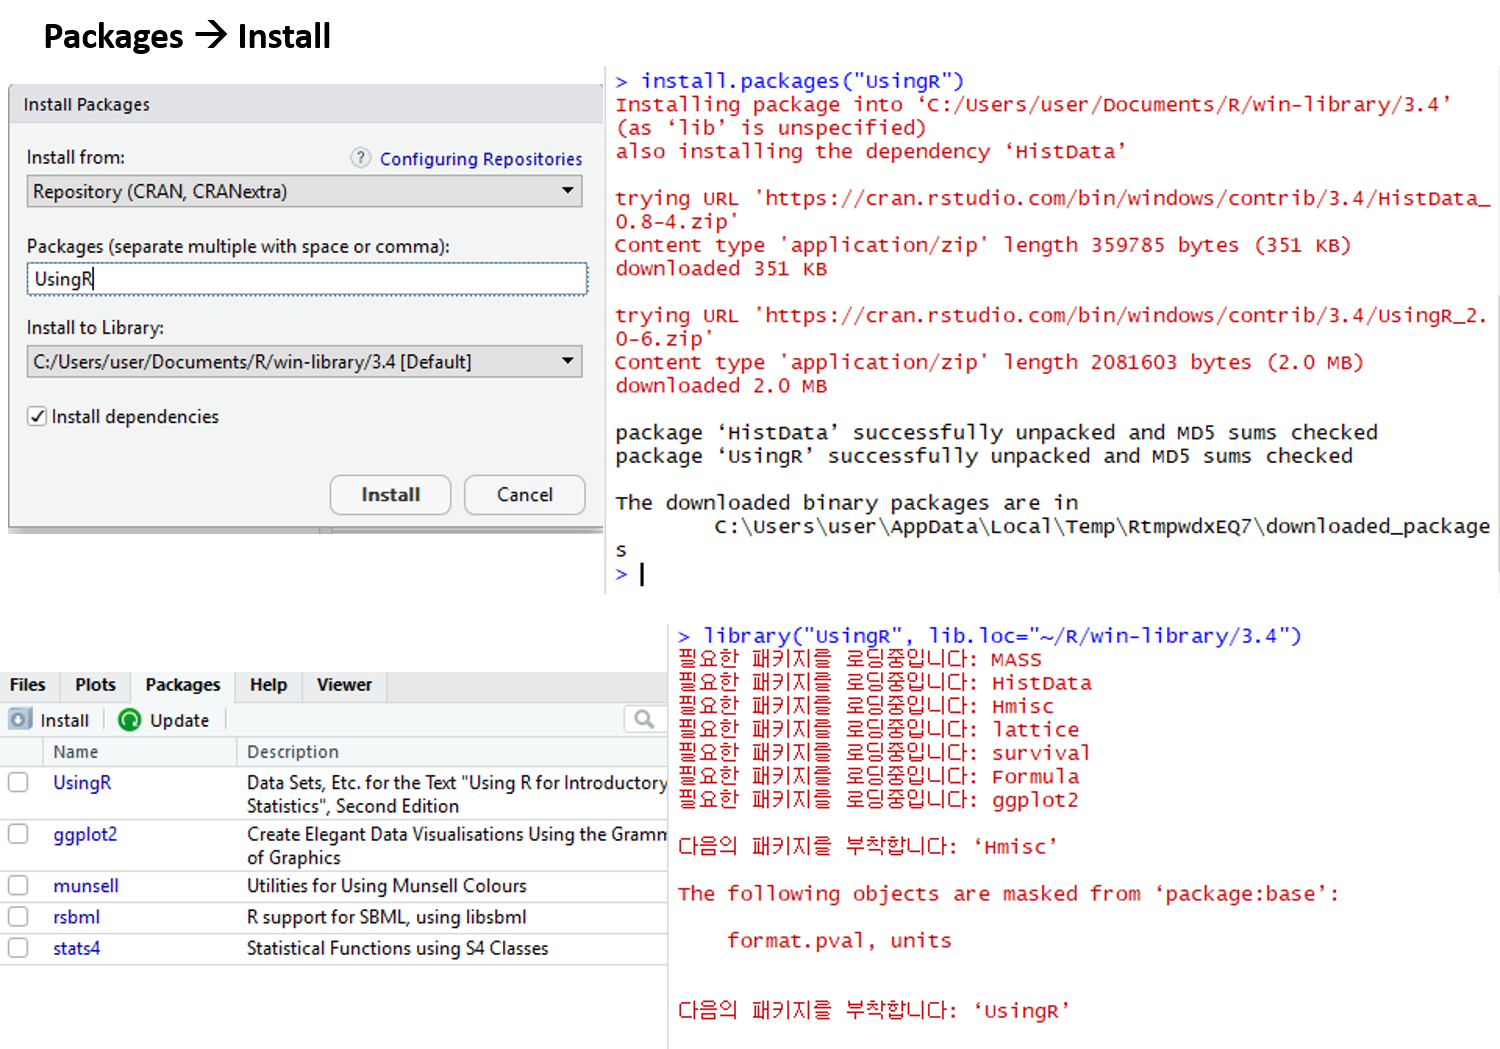
\includegraphics[width=3.64583in,height=\textheight]{images/01/01-19.png}

\begin{Shaded}
\begin{Highlighting}[]
\FunctionTok{install.packages}\NormalTok{(}\StringTok{"UsingR"}\NormalTok{)}
\end{Highlighting}
\end{Shaded}

\begin{itemize}
\tightlist
\item
  UsingR package loading
\end{itemize}

\begin{Shaded}
\begin{Highlighting}[]
\FunctionTok{library}\NormalTok{(UsingR)}
\FunctionTok{help}\NormalTok{(}\AttributeTok{package=}\StringTok{"UsingR"}\NormalTok{)}
\end{Highlighting}
\end{Shaded}

일반적으로 패키지 안에 관련된 데이터도 같이 저장되어 있으며 \texttt{data()} 함수를 이용해서 패키지 데이터를 사용자 작업공간에 복사해서 사용 가능합니다.

\begin{Shaded}
\begin{Highlighting}[]
\FunctionTok{head}\NormalTok{(rivers)}
\FunctionTok{length}\NormalTok{(rivers)}
\FunctionTok{class}\NormalTok{(rivers)}
\FunctionTok{data}\NormalTok{(rivers)}
\FunctionTok{data}\NormalTok{(}\AttributeTok{package=}\StringTok{"UsingR"}\NormalTok{)}
\FunctionTok{library}\NormalTok{(HistData)}
\FunctionTok{head}\NormalTok{(Cavendish)}
\FunctionTok{str}\NormalTok{(Cavendish)}
\FunctionTok{head}\NormalTok{(Cavendish}\SpecialCharTok{$}\NormalTok{density2)}
\end{Highlighting}
\end{Shaded}

\hypertarget{r-programming}{%
\section{R programming}\label{r-programming}}

\hypertarget{console-calculator}{%
\subsection{Console calculator}\label{console-calculator}}

\begin{Shaded}
\begin{Highlighting}[]
\DecValTok{2} \SpecialCharTok{+} \DecValTok{2}
\NormalTok{((}\DecValTok{2}\NormalTok{ – }\DecValTok{1}\NormalTok{)}\SpecialCharTok{\^{}}\DecValTok{2} \SpecialCharTok{+}\NormalTok{ (}\DecValTok{1}\NormalTok{ – }\DecValTok{3}\NormalTok{)}\SpecialCharTok{\^{}}\DecValTok{2}\NormalTok{ )}\SpecialCharTok{\^{}}\NormalTok{(}\DecValTok{1}\SpecialCharTok{/}\DecValTok{2}\NormalTok{)}
\DecValTok{2} \SpecialCharTok{+} \DecValTok{2}\NormalTok{; }\DecValTok{2} \SpecialCharTok{{-}} \DecValTok{2}
\end{Highlighting}
\end{Shaded}

\hypertarget{exercise-1}{%
\subsection{Exercise}\label{exercise-1}}

다음 공식들을 계산하는 R 코드를 작성하시오

\[ \sqrt{(4+3)(2+1)} \]

\[ 2^3 + 3^2 \]

\[ \frac{0.25 - 0.2}{\sqrt{0.2 (1-0.2)/100}}\]

\hypertarget{variables-and-values}{%
\subsection{Variables and values}\label{variables-and-values}}

\begin{itemize}
\tightlist
\item
  프로그래밍 언어의 공통적 개념 \texttt{변수}, \texttt{함수}, \texttt{자료형}, \texttt{조건문}, \texttt{반복문}\\
\item
  Assignment operator ( \texttt{\textless{}-} OR \texttt{=} )

  \begin{itemize}
  \tightlist
  \item
    Valid object name \texttt{\textless{}-} value
  \item
    단축키: \texttt{Alt\ +\ -} (the minus sign)
  \end{itemize}
\end{itemize}

\begin{Shaded}
\begin{Highlighting}[]
\NormalTok{x }\OtherTok{\textless{}{-}} \DecValTok{2}
\NormalTok{y }\OtherTok{\textless{}{-}}\NormalTok{ x}\SpecialCharTok{\^{}}\DecValTok{2}\NormalTok{ – }\DecValTok{2}\SpecialCharTok{*}\NormalTok{x }\SpecialCharTok{+} \DecValTok{1}
\NormalTok{y}
\NormalTok{x }\OtherTok{\textless{}{-}} \StringTok{"two"}  
\NormalTok{some\_data }\OtherTok{\textless{}{-}} \FloatTok{9.8}
\end{Highlighting}
\end{Shaded}

\begin{itemize}
\tightlist
\item
  내장 변수 Built-in variables
\end{itemize}

\begin{Shaded}
\begin{Highlighting}[]
\NormalTok{pi}
\end{Highlighting}
\end{Shaded}

\begin{itemize}
\tightlist
\item
  변수이름 작명법

  \begin{itemize}
  \tightlist
  \item
    문자, 숫자, ``\_'', ``.'' 등으로 구성
  \item
    대소문자 구분
  \item
    가독성, 의미있는 변수 이름
  \item
    길이 제한 없음
  \end{itemize}
\end{itemize}

\begin{Shaded}
\begin{Highlighting}[]
\NormalTok{i\_use\_snake\_case }\OtherTok{\textless{}{-}} \DecValTok{1}
\NormalTok{otherPeopleUseCamelCase }\OtherTok{\textless{}{-}} \DecValTok{2}
\NormalTok{some.people.use.periods }\OtherTok{\textless{}{-}} \DecValTok{3}
\NormalTok{And\_aFew.People\_RENOUNCEconvention }\OtherTok{\textless{}{-}} \DecValTok{4}
\end{Highlighting}
\end{Shaded}

\begin{itemize}
\tightlist
\item
  자동 완성 기능 (Tab completion) in RStudio
\item
  이전 명령은 콘솔에서 위 아래 화살표
\end{itemize}

\hypertarget{exercise-2}{%
\subsection{Exercise}\label{exercise-2}}

\begin{enumerate}
\def\labelenumi{\arabic{enumi}.}
\item
  변수 \texttt{x}에 1, 3, 5, 7, 9를, 변수 \texttt{y}에 2, 4, 6, 8, 10을 저장하는 코드를 작성하시오
\item
  앞서 변수 \texttt{x}와 \texttt{y}를 더한 값을 \texttt{z}에 저장하는 코드를 작성하시오
\item
  변수 x에 ``hello world!'' 를 저장하고 x의 값을 출력하는 코드를 작성하시오
\end{enumerate}

\hypertarget{functions}{%
\subsection{Functions}\label{functions}}

함수(Function)란 사용자가 원하는 기능을 수행하는 코드의 모음으로서 반복적으로 쉽게 사용할 수 있도록 만들어 놓은 코드 입니다. 특정 데이터를 입력으로 받아 원하는 기능을 수행한 후 결과 데이터를 반환하는 구조를 가집니다. 함수는 일반적으로 다음과 같은 포멧으로 구현할 수 있습니다.

\begin{Shaded}
\begin{Highlighting}[]
\NormalTok{my\_function\_name }\OtherTok{\textless{}{-}} \ControlFlowTok{function}\NormalTok{(parameter1, parameter2, ... )\{}
  \DocumentationTok{\#\#any statements}
  \FunctionTok{return}\NormalTok{(object)}
\NormalTok{\}}
\end{Highlighting}
\end{Shaded}

예를 들어 다음과 같은 \texttt{my\_sine} 함수를 만들 수 있으며 parameter (매개변수)는 \texttt{x}이고 \texttt{y}는 반환값을 저장하는 지역변수 입니다.

\begin{Shaded}
\begin{Highlighting}[]
\NormalTok{my\_sine }\OtherTok{\textless{}{-}} \ControlFlowTok{function}\NormalTok{(x)\{}
\NormalTok{    y }\OtherTok{\textless{}{-}} \FunctionTok{sin}\NormalTok{(x)}
    \FunctionTok{return}\NormalTok{(y)}
\NormalTok{\}}
\end{Highlighting}
\end{Shaded}

\begin{itemize}
\tightlist
\item
  내장 함수 (Built-in functions)
\end{itemize}

\begin{Shaded}
\begin{Highlighting}[]
\NormalTok{x }\OtherTok{\textless{}{-}}\NormalTok{ pi}
\FunctionTok{sin}\NormalTok{(x)}
\FunctionTok{sqrt}\NormalTok{(x)}
\FunctionTok{log}\NormalTok{(x)}
\FunctionTok{log}\NormalTok{(x, }\DecValTok{10}\NormalTok{)}
\NormalTok{x }\OtherTok{\textless{}{-}} \FunctionTok{c}\NormalTok{(}\DecValTok{10}\NormalTok{, }\DecValTok{20}\NormalTok{, }\DecValTok{30}\NormalTok{)}
\NormalTok{x }\SpecialCharTok{+}\NormalTok{ x}
\FunctionTok{mean}\NormalTok{(x)}
\FunctionTok{sum}\NormalTok{(x)}\SpecialCharTok{/}\FunctionTok{length}\NormalTok{(x)}
\end{Highlighting}
\end{Shaded}

\hypertarget{exercise-3}{%
\subsection{Exercise}\label{exercise-3}}

\begin{enumerate}
\def\labelenumi{\arabic{enumi}.}
\item
  변수 \texttt{x}에 1, 3, 5, 7, 9를, 변수 \texttt{y}에 2, 4, 6, 8, 10을 저장하는 코드를 작성하시오
\item
  \texttt{x}와 \texttt{y}를 더한 값을 \texttt{z}에 저장하는 코드를 작성하시오
\item
  \texttt{mysum} 이라는 이름의 함수를 작성하되 두 변수를 입력으로 받아 더한 후 결과를 반환하는 코드를 작성하시오
\item
  \texttt{mymean} 이라는 이름의 함수를 작성하되 두 변수를 입력으로 받아 평균을 구한 후 결과를 반환하는 코드를 작성하시오
\end{enumerate}

이 저작물은 크리에이티브 커먼즈 저작자표시-비영리-변경금지 4.0 국제 라이선스에 따라 이용할 수 있습니다.

  \bibliography{book.bib,packages.bib}

\end{document}
